%%%%%%%%%%%%%%%%%%%%%%%%%%%%%%%%%
%% Ersetzen Sie in den folgenden Zeilen die entsprechenden -Texte-
%% mit den richtigen Werten.
\documentclass[course=erap]{aspdoc}
\newcommand{\theGroup}{155} % Beispiel: 42
\newcommand{\theNumber}{A501} % Beispiel: A123
\author{Mete Polat \and Jonas Hübotter \and Simon Martin Bohnen}
\date{Sommersemester 2019} % Beispiel: Wintersemester 2018/19
%%%%%%%%%%%

\usepackage{amssymb}
\usepackage{biblatex}
\addbibresource{Literatur.bib}

% Diese Zeile bitte -nicht- aendern.
\title{Gruppe \theGroup{} -- Abgabe zu Aufgabe \theNumber}

\begin{document}
\maketitle

\section{Einleitung}


\section{Problemstellung und Spezifikation}


\section{Lösungsfindung}


\section{Dokumentation der Implementierung}


\section{Ergebnisse}

\subsection{Sicherheit}

\subsection{Feistelchiffren}

Die folgende allgemeine Darstellung von Feistelchiffren soll auf klassische (auch ausgewogene) Feistelchiffren begrenzt werden. Wie für RC5, gilt für klassische Feistelchiffren, dass die Längen der beiden Halbblöcke eines Blocks gleich sein müssen. Zudem wird sich auf das für die umkehrbare Verknüpfung von zwei Halbblöcken übliche $\oplus$ (XOR) beschränkt.

\subsubsection{Einrundige Feistelnetzwerke}

Eine Feistelchiffre ist eine rundenbasierte Blockchiffre, die nach der Art eines Feistelnetzwerks aufgebaut ist. Sei
\[
    F_n := \{f \mid f \colon \{0,1\}^n \to \{0,1\}^n\}
\]
die Famile der Rundenfunktionen. Zunächst soll ein klassisches einrundiges Feistelnetzwerk $\Psi$ betrachtet werden. Dieses wird definiert durch eine beliebige Abbildung $f \in F_n$ und eine umkehrbare Bitoperation --- durch obige Einschränkung der Allgemeinheit $\oplus$.
\[
    \Psi(f) \colon \{0,1\}^{2n} \to \{0,1\}^{2n} \colon [L, R] \mapsto [S, T] \Leftrightarrow
        \begin{cases}
            S = R \\
            T = L \oplus f(R) \\
        \end{cases}
\]
für $\forall(L,R) \in (\{0,1\}^n)^2$.\cite[p.11]{nachef}

\begin{center}
    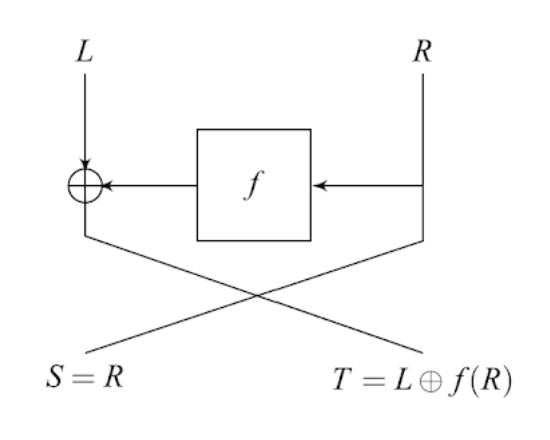
\includegraphics[scale=1]{img/1_round_feistel_cipher_enc.png}\break
    \cite[Fig. 2.1]{nachef}
\end{center}

Wichtig für jede Verschlüsselung ist Bijektivität, damit jedem Codewort eine eindeutige Plaintext-Nachricht zugeordnet werden kann. $\Psi(f)$ ist unabhängig von $f \in F_n$ eine Permutation, d.h. $f$ selbst muss nicht bijektiv sein.\cite[p.12]{nachef}\bigbreak

Aus der Definition von $\Psi(f)$ ergibt sich ihr Inverses als
\[
    \Psi(f)^{-1} = \sigma \circ \Psi(f) \circ \sigma
\]
mit $\sigma$ definiert als $\sigma([L,R]) = [R,L]$ für $L,R \in \{0,1\}^n$, der Vertauschung beider Halbblöcke.\cite[p.12]{nachef}

\begin{center}
    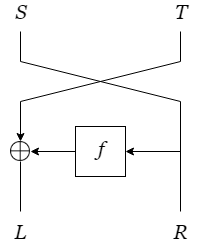
\includegraphics[scale=0.5]{img/1_round_feistel_cipher_dec.png}
\end{center}

\subsubsection{r-rundige Feistelnetzwerke}

Üblicherweise werden Feistelnetzwerke in mehreren Runden angewendet. Im Allgemeinen ist ein klassisches Feistelnetzwerk mit $r \geq 1$ Runden und $f_1,f_2,...,f_r \in F_n$ Rundenfunktionen definiert durch
\[
    \Psi^r(f_1,...,f_r) = \Psi(f_r) \circ ... \circ \Psi(f_2) \circ \Psi(f_1).
\]\cite[p.12]{nachef}

\begin{center}
    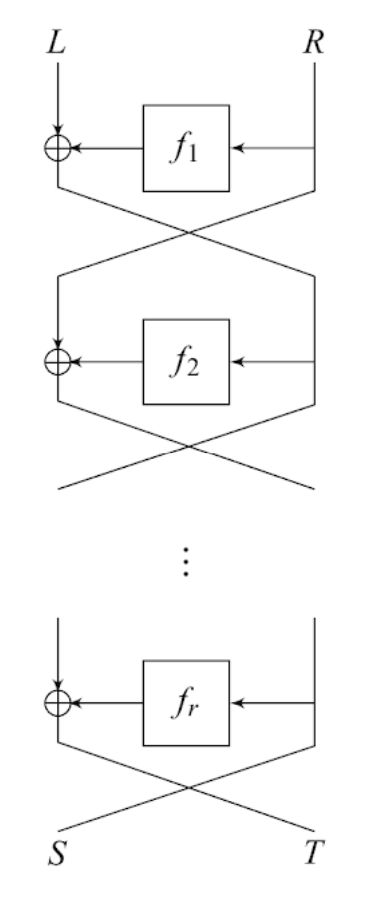
\includegraphics[scale=1]{img/r_round_feistel_cipher_enc.png}\break
    \cite[Fig. 2.2]{nachef}
\end{center}

Da ein einrundiges Feistelnetzwerk eine Permutation über $\{0,1\}^{2n}$ ist, sind auch $r$-rundige Feistelnetzwerke Permutationen. Weiterhin ist das Inverse eines $r$-rundigen Feistelnetzwerks die Komposition der Inversen der einzelnen Runden.
\begin{align*}
    (\Psi^r(f_1,...,f_r))^{-1} &= \sigma \circ \Psi(f_1) \circ \sigma \circ ... \circ \sigma \circ \Psi(f_r) \circ \sigma  \\
                               &= \sigma \circ \Psi^r(f_r,...,f_1) \circ \sigma
\end{align*}\cite[p.13]{nachef}\bigbreak

Eine Feistelchiffre ist nun ein spezielles Feistelnetzwerk, dessen Rundenfunktionen von einem Rundenschlüssel aus dem Schlüsselraum $K$ abhängen.
Seien die Rundenschlüssel $(k_1,...,k_r) \in K^r$ und die Familie der Rundenfunktionen
\[
    F_{n,K} := \{f_k \mid k \in K, f_k \colon \{0,1\}^n \to \{0,1\}^n\}.
\]
Dann ist eine Feistelchiffre das Feistelnetzwerk $\Psi^r(f_{k_1},...,f_{k_r})$. Also die $r$-rundige Permutation von der Nachricht $\{0,1\}^{2n}$ in Abhängigkeit vom Schlüssel $(k_1,...,k_r)$.\cite[p.14]{nachef}

\subsubsection{RC5 als Feistelchiffre}

RC5 ist eine symmetrische Blockchiffre, deren Aufbau dem einer Feistelchiffre gleicht. RC5 hat die Parameter:

\begin{itemize}
    \item $w$ ist die Wortgröße in Bits. Ein durch RC5 verschlüsselbarer Block besteht aus zwei Wörtern.
    \item $r$ ist die Anzahl der Runden in denen RC5 Operationen auf einem Block ausführt. Jede Runde besteht aus zwei Halbrunden, in denen ein Wort aus dem Block alteriert wird.
    \item $b$ ist die Anzahl der Bytes in dem privaten Schlüssel $K$.
\end{itemize}

RC5 baut zu Beginn die erweiterte Schlüsseltabelle $S$ auf, die aus $2r + 2$ Schlüsseln besteht und von $K$ abhängt. Seien $\Sigma := (S_2,S_3,...,S_{2r+1}) = (\Sigma_0,\Sigma_1,...,\Sigma_{2r-1})$ mit $|\Sigma| = 2r$ die Schlüssel aus der erweiterten Schlüsseltabelle, die während der Runden von RC5 zum Verschlüsseln benutzt werden --- $S_0$ und $S_1$ werden für das Key-Whitening genutzt. Zudem sei $(g_{\Sigma_0},g_{\Sigma_1},...,g_{\Sigma_{2r-1}})$ definiert durch
\begin{align*}
    g_k \colon &\{0,1\}^w \times \{0,1\}^w \to \{0,1\}^w \colon \\
               &(\tau, R) \mapsto (\tau \lll R) + k
\end{align*}
mit $\tau = L \oplus R$, $k \in \Sigma$ und $L, R \in \{0,1\}^w$ wobei $x \lll y$ die Linksrotation von $x$ um $y$ Bits angibt. Dann zeigt die folgende Tabelle die Zusammenhänge von RC5 und Feistelchiffren.

\begin{center}
 \begin{tabular}{c|c}
 RC5 & Feistelchiffre \\
 \hline
 $r$ & $2r$ \\
 $w$ & $n$ \\
 $\Sigma$ & $K^{2r}$ \\
 $(g_{\Sigma_0},g_{\Sigma_1},...,g_{\Sigma_{2r-1}})$ & $(f_{k_1},...,f_{k_{2r}}) \in F^{2r}_{n,K}$ \\
\end{tabular}
\end{center}

Die Reihenfolge der Anwendung der umkehrbaren Bitoperation ($\oplus$) und der Rundenfunktion unterscheidet sich leicht zwischen RC5 und einer allgemeinen klassischen Feistelchiffre. Dieser Unterschied soll in der folgenden Abbildung skizziert werden.

\begin{samepage}
\begin{center}
    \includegraphics[scale=0.5]{img/rc5_feistel_cipher.png}\break
    \textit{Links eine Runde einer Feistelchiffre, rechts eine Runde (zwei Halbrunden) von RC5.}
\end{center}
\end{samepage}

wobei $r$ die aktuelle Runde angibt. Wie dargestellt, ist eine Halbrunde von RC5 im Aufbau ähnlich zu einer Runde einer Feistelchiffre.\bigbreak

Durch den leicht modifizierten Aufbau einer Feistelchiffre in RC5, verändert sich bei RC5 die Berechnung der Inversen. Für eine RC5-Runde gilt
\[
    RC5_{r,\Sigma} \colon \{0,1\}^{2w} \to \{0,1\}^{2w} \colon [L, R] \mapsto [S, T] \Leftrightarrow
        \begin{cases}
            S = ((L \oplus R) \lll R) + \Sigma_{2r-2} \\
            T = ((R \oplus S) \lll S) + \Sigma_{2r-1} \\
        \end{cases}.
\]
Damit gilt für die Berechnung der Inversen von einer RC5-Runde
\[
    RC5_{r,\Sigma}^{-1} \colon \{0,1\}^{2w} \to \{0,1\}^{2w} \colon [S, T] \mapsto [L, R] \Leftrightarrow
        \begin{cases}
            L = ((S - \Sigma_{2r-2}) \ggg R) \oplus R \\
            R = ((T - \Sigma_{2r-1}) \ggg S) \oplus S \\
        \end{cases}
\]
für $\forall(S, T) \in (\{0,1\}^w)^2$ wobei $x \ggg y$ die Rechtsrotation von $x$ um $y$ Bits angibt.

\subsection{PKCS\#7-Padding}

Da eine Blockchiffre nur Nachrichten vollständig verschlüsseln kann, die restfrei in Blöcke geteilt werden können, muss die Länge dieser Nachrichten zunächst auf ein Vielfaches der Blockgröße erweitert werden. Diese Erweiterung wird im Allgemeinen als Padding bezeichnet.\bigbreak

Das PKCS\#7-Padding ist eine Form der Erweiterung des Plaintextes auf ein Vielfaches der Blocklänge und soll im Folgenden erläutert werden. Es sei $\Delta$ definiert als
\[
    \Delta = b - (l \bmod b)
\]
mit $b$ als der Länge eines Blocks und $l$ als der Länge des Plaintextes in Byte. Vor der Anwendung eines Verschlüsselungsalgorithmus, der als Länge des Inputs ein Vielfaches von $b$ Bytes erwartet, werden $\Delta$ Bytes jeweils mit dem Wert $\Delta$ an den Plaintext angefügt.\cite[p.28]{rfc5652}\bigbreak

Das heißt, dass der Input in Abhängigkeit von $b$ und $l$ um eine der folgenden Byte-Sequenzen erweitert wird:

\begin{samepage}
\begin{verbatim}
                     01 -- if l mod b = b-1
                  02 02 -- if l mod b = b-2
                      .
                      .
                      .
            b b ... b b -- if l mod b = 0
\end{verbatim}
\end{samepage}

Nach dem Entschlüsseln des Codewortes, kann das Padding auf eindeutige Weise entfernt werden, da jeder Plaintext --- einschließlich jener, deren Länge selbst ein Vielfaches der Blockgröße ist --- vor der Verschlüsselung mit PKCS\#7-Padding erweitert wurde. Die Anzahl der zu entfernenden Bytes wird durch das letzte Byte des letzten Blocks angegeben. PKCS\#7-Padding ist wohldefiniert für $b < 256$.\cite[p.28]{rfc5652}

\subsection{Performance}

\section{Zusammenfassung}

\printbibliography

\end{document}

